\chapter{Recognizing Human Activities from Partially Observed Videos}

\section{Introduction}
Human activity recognition aims at building robust and efficient computer
vision algorithms and systems which can automatically recognize specific human
activities from a sequence of video frames. Its applications include security,
surveillance and human-computer interaction, etc.  Early research on this
problem
~\cite{ActionsAsSpaceTimeShapes_iccv05,DollarVSPETS05cuboids,lifeifei2008,STIP2008,christian2004}
focused on a single person's simple actions, such as walking, running, and
hopping. Recently, research on activity recognition has been extended to more
complex activity scenarios which involve multiple persons interacting with each
other or objects~\cite{Ryoo2009,Waltisberg_variationsof,Tsz-Ho2010}.

One widely used approach for human activity recognition is to train and
classify the spatiotemporal features extracted from videos with different
activities. Inspired by successful 2D scale-invariant image feature
descriptors~\cite{SIFT2004,HOG2005}, a variety of spatiotemporal feature
detectors/descriptors have been
developed~\cite{STIP2008,DollarVSPETS05cuboids,Jhuang07abiologically,Laptev03space-timeinterest,GeertECCV2008,Shu-FaiICCV2007},
and their robustness and {\color{black}effectiveness} have been demonstrated in
several successful human activity recognition
methods~\cite{DollarVSPETS05cuboids,lifeifei2008,STIP2008,christian2004,Ryoo2009,Ryoo2011,Waltisberg_variationsof,Klaser_aspatio-temporal,Scovanner07icm}.
In these methods, a sequence of 2D video frames are treated as a 3D XYT video
volume {\color{black} in which} interest points are located by finding local
maxima in the responses of the feature detector, followed by calculating
vectorized feature descriptors at each interest point.  By using the
bag-of-visual-words technique, spatiotemporal features within a video can be
combined into a feature vector that describes the activity
{\color{black}presented} in the video.

\begin{figure}[htbp]
  \begin{center}
    \epsfig{file=figures/problem_illustration.eps,width=0.95\linewidth}\quad
  \end{center}
  \vspace{-4mm}
  \caption{An illustration of the human activity recognition from fully and partially observed videos.}
  \vspace{-4mm}
  \label{fig:problem_illustration}
\end{figure}
Previous research on human activity recognition usually focused on recognizing
activities after fully observing the entire video, as illustrated in
Fig.~\ref{fig:problem_illustration}(a).  However in practice, partially
observed videos may occur when video signals drop off, cameras or objects of
interest are occluded, or videos are composited from multiple sources. The
unobserved subsequence may occur any time with any duration, yielding a
temporal gap as shown in Fig.~\ref{fig:problem_illustration}(c).  Recognizing
activities in such temporal gaps is of particular importance in defense and
security. For example, one of the four major themes in the DARPA Mind's Eye
program\footnote{\url{http://www.darpa.mil/Our_Work/I2O/Programs/Minds_Eye.aspx}}
is to handle such gapped videos for activity recognition.

When the unobserved subsequence is at the end of the video, the problem is
{\color{black} reduced} to activity prediction from unfinished activity
streaming, as illustrated in Fig.~\ref{fig:problem_illustration}(b).  Activity
prediction has been studied by Ryoo~\cite{Ryoo2011}. Another example of related
work on activity prediction is the max-margin early event detectors
(MMED)~\cite{MMED2012}, which try to detect the temporal location and duration
of a certain activity from the video streaming. {\color{black}Recently, Kitani
  \etal studied a special activity prediction problem
  in~\cite{Kitani_2012_7250}, which tries to predict the walking path of a
  person in certain environments based on historical data}. However, activity
recognition from general gapped videos, as shown in
Fig.~\ref{fig:problem_illustration}(c), has not been well studied yet.  Note
that, in general, this is a different problem from activity prediction because
the temporal gap may divide the video into two disjoint observed video
subsequences and we need to combine them to achieve a reliable recognition.

In this paper, we propose a probabilistic formulation for human activity
recognition from partially observed videos, where the posterior is maximized
for the recognized activity class and the observed video frames. In our
formulation, the key component in defining the posterior is the likelihood that
the observed video frames describe a certain class of activity. In this paper,
we take a set of training video samples (completely observed) of each activity
class as the bases, and then use sparse coding (SC) to derive the likelihood
that a certain {\color{black} type of }activity is presented in a partially
observed test video.  Furthermore, we divide each activity into multiple
temporal segments, apply sparse coding to derive the activity likelihood at
each segment, and finally combine the likelihoods at each segment to achieve a
global posterior for the activity. While video segments are constructed by
uniformly dividing the video in SC, we also extend it to include more sparse
coding bases constructed from a mixture of training video segments (MSSC) with
different lengths and locations.

Using sparse coding with the constructed bases, the proposed methods can find
closest video segments from different training videos when matching a new test
video. Thus, the proposed methods don't require full temporal alignment between
any pair of (training or test) videos, and they can handle the problems of 1) a
limited number of training videos; 2) possible outliers in the training video
data; and 3) large intra-class variations. We evaluate the proposed methods on
several video datasets and compare their performance with several
state-of-the-art methods.  In the experiments, we not only evaluate the
performance on general gapped videos, but also on fully observed videos without
a gap and videos with a gap at the end (activity prediction).

The remainder of the paper is organized as follows. In
Section~\ref{sec:problem_formulation}, we present our probabilistic formulation
of human activity recognition from partially observed
videos. Section~\ref{sec:likelihood} introduces the likelihood component using
a sparse coding (SC) technique followed by extending the SC to include more
bases constructed from a mixture of segments (MSSC) with different temporal
lengths.  Experimental results and discussions are presented in
Section~\ref{sec:experiments}, followed by conclusions in
Section~\ref{sec:conclusion}.

% -------------------------------------------------------------------------
\section{Problem Formulation}\label{sec:problem_formulation}

\subsection{Human Activity Recognition from a Fully Observed Video}
\label{sec:complete}
Given a fully observed video $\mathcal{O}[1:T]$ of length $T$, where
$\mathcal{O}[t]$ indicates the frame at time $t$, the goal is to classify the
video $\mathcal{O}[1:T]$ into one of $P$ activity classes $\mathcal{A} =
\{\mathcal{A}_p\}, p=1,\dots,\mathcal{P}$. A human activity is usually made up
of a sequence of simpler actions, each of which may contain different
spatiotemporal features.  Therefore, we can divide the video $\mathcal{O}[1:T]$
into a sequence of shorter video \textit{segments} for spatiotemporal feature
extraction. For simplicity, we uniformly divide the video $\mathcal{O}[1:T]$
into $M$ equal-length segments, where each segment $\mathcal{O}(t_{i-1}:t_i]$,
with $t_i=\frac{iT}{M}$, corresponds to the $i$-th stage of the activity, with
$i=1,2,\cdots, M$.  For different videos, the length $T$ might be different,
and therefore the segments from different videos may have different lengths.

The posterior probability that an activity $\mathcal{A}_p$ is presented in the
video $\mathcal{O}[1:T]$ can be defined as $P(\mathcal{A}_p |
\mathcal{O}[1:T])$, which can be rewritten as:
\begin{equation}
  \label{eq:full_observed_formulation}
  \begin{split}
    P(&\mathcal{A}_p | \mathcal{O}[1:T])\propto \sum_{i=1}^M P(\mathcal{A}_p, (t_{i-1}:t_i] | \mathcal{O}[1:T]) \\
    &\propto \sum_{i=1}^M P(\mathcal{A}_p, (t_{i-1}:t_i])P(\mathcal{O}[1:T] | \mathcal{A}_p, (t_{i-1}:t_i]).
  \end{split}
\end{equation}
In this formulation, $P(\mathcal{A}_p, (t_{i-1}:t_i])$ is the prior of stage
$i$ of activity $\mathcal{A}_p$ and $P(\mathcal{O}[1:T] | \mathcal{A}_p,
(t_{i-1}:t_i])$ is the observation likelihood given activity class
$\mathcal{A}_p$ in the $i$-th stage. Then the index of the recognized activity
is
\begin{equation}
  \begin{split}
    p^* = \arg\max_p  \sum_{i=1}^M &P(\mathcal{A}_p, (t_{i-1}:t_i]) \cdot \\
    &P(\mathcal{O}[1:T] | \mathcal{A}_p, (t_{i-1}:t_i]).
  \end{split}
\end{equation}

\subsection{Human Activity Recognition from a Partially Observed Video}
\label{sec:incomplete}
A partially observed video can be represented by $\mathcal{O}[1:T_1]\cup
\mathcal[T_2:T]$, where frames $\mathcal{O}(T_1:T_2)$ are missing, as
illustrated in Fig.~\ref{fig:formulation_illustration}.  For simplicity, we
assume that $T_1$ is always the last frame of a segment and $T_2$ is always the
first frame of another segment. Otherwise, we can intentionally decrease $T_1$
to a nearest last frame of a segment and increase $T_2$ to a nearest first
frame of a segment.

\begin{figure}[htbp]
  \begin{center}
    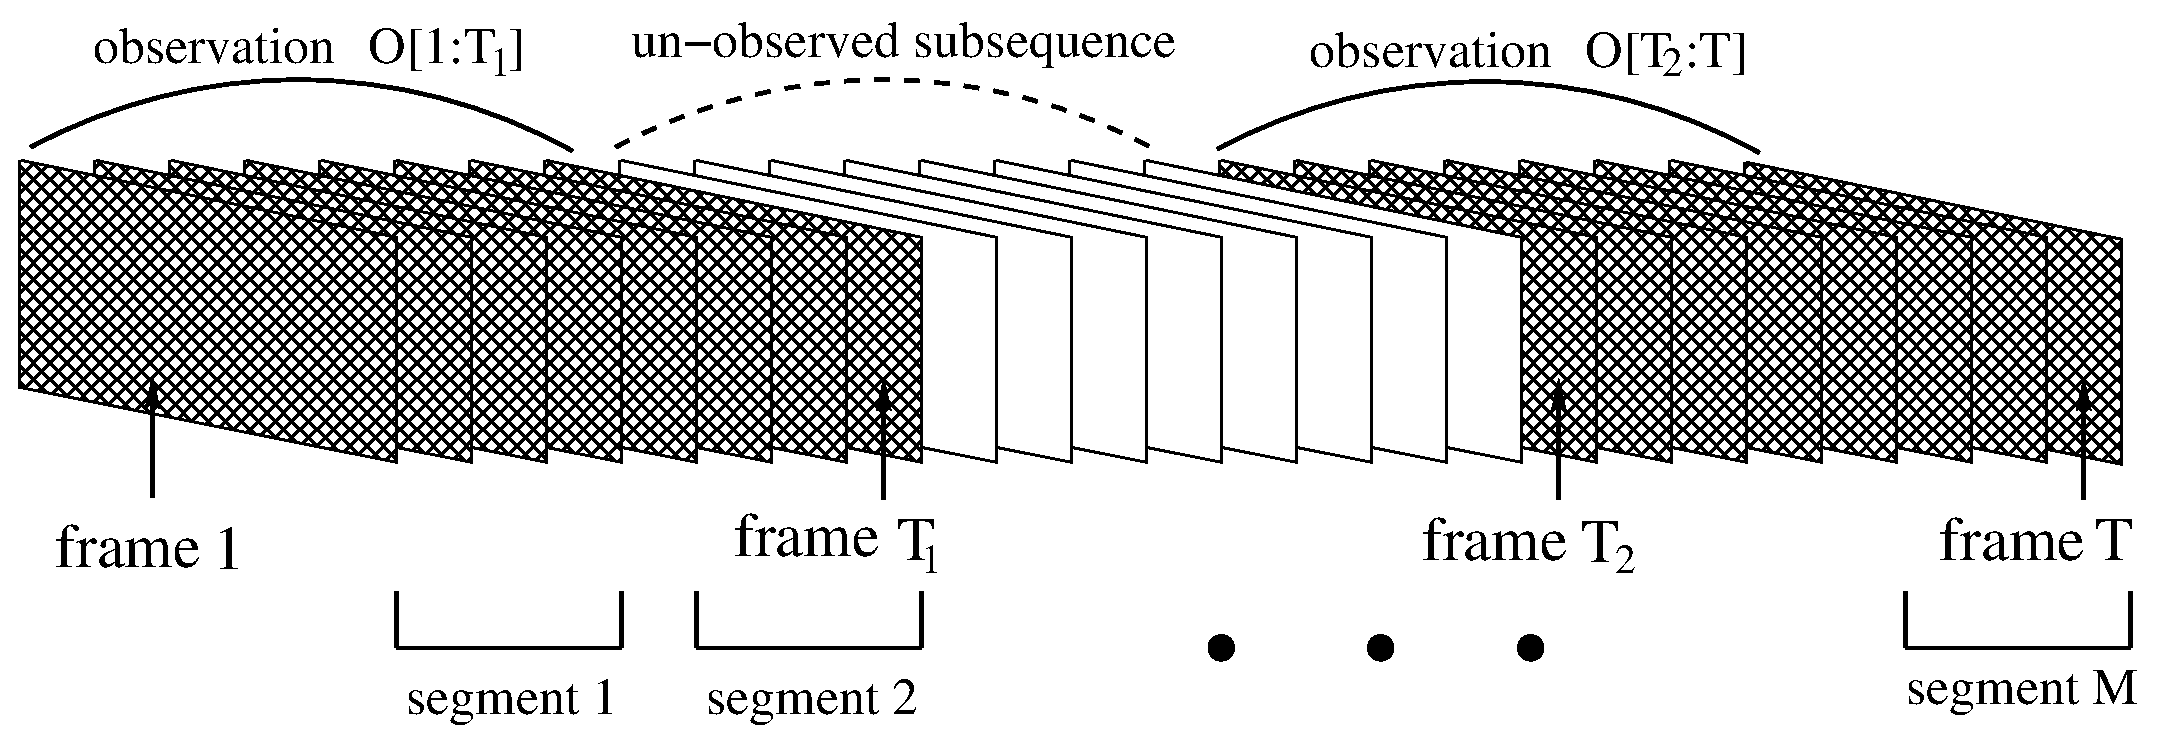
\epsfig{file=figures/formulation_illustration.eps,width=1.0\linewidth}
  \end{center}
  \vspace{-4mm}
  \caption{An illustration of a partially observed video (general case), where the
    unobserved subsequence is located in the middle of the video.}
  \label{fig:formulation_illustration}
  \vspace{-2mm}
\end{figure}
By following the formulation in Eqn.~(\ref{eq:full_observed_formulation}), the
posterior probability that an activity $\mathcal{A}_p$ is presented in this
partially observed video can be defined as:
\begin{equation}
  \begin{split}
    P(\mathcal{A}_p& | \mathcal{O}[1:T_1]\cup \mathcal{O}[T_2:T]) \propto \\
    & \omega_1  \sum_{i|t_i\leq T_1} P(\mathcal{A}_p, (t_{i-1}:t_i] | \mathcal{O}[1:T_1])   \\
    & + \omega_2 \sum_{i|t_{i-1}\geq T_2} P(\mathcal{A}_p, (t_{i-1}:t_i] | \mathcal{O}[T_2:T]),
  \end{split}
\end{equation}
where $\omega_1=\frac{T_1}{T_1+T-T_2+1}$ and
$\omega_2=\frac{T-T_2+1}{T_1+T-T_2+1}$ reflect the proportionality between the
length of $\mathcal{O}[1:T_1]$ and $\mathcal{O}[T_2:T]$.  We can rewrite this
as:
\begin{equation}
  \begin{split}
    &P(\mathcal{A}_p | \mathcal{O}[1:T_1]\cup \mathcal{O}[T_2:T])  \propto \\
    &\omega_1  \sum_{i|t_i\leq T_1} P(\mathcal{A}_p, (t_{i-1}:t_i])P(\mathcal{O}[1:T_1]|\mathcal{A}_p, (t_{i-1}:t_i]) \\
    &+\omega_2  \sum_{i|t_{i-1}\geq T_2} P(\mathcal{A}_p, (t_{i-1}:t_i])P(\mathcal{O}[T_2:T]|\mathcal{A}_p, (t_{i-1}:t_i]).
  \end{split}
  \label{Eq:full-likelihood}
\end{equation}
The index of the recognized activity is therefore:
\begin{equation}
  p^* = \arg\max_p P(\mathcal{A}_p | \mathcal{O}[1:T_1]\cup \mathcal{O}[T_2:T]).
  \label{eq:maximization}
\end{equation}
Notably, when $T_2-1 = T$ the problem is {\color{black}reduced} to
{\color{black}its special case -- activity prediction}.  When $T_1 = T$, the
problem is degenerated to the classic human activity recognition from fully
observed videos.  {\color{black}In practice}, we can assume that the prior of
$\mathcal{A}_p$ on each segment satisfies a uniform distribution, without
favoring any special activity.  We introduce the calculation of the likelihood
component in the following section.

%% =======================================================================================
\section{Likelihood}
\label{sec:likelihood}

\subsection{Likelihood calculation using sparse coding}
\label{sec:likelihood_SC}
Without loss of generality, in this section, we only consider the calculation
of the likelihood $P(\mathcal{O}[1:T_1]|\mathcal{A}_p, (t_{i-1}:t_i])$, since
$P(\mathcal{O}[T_2:T]|\mathcal{A}_p, (t_{i-1}:t_i])$ can be calculated in a
similar way. The basic idea is to collect a set of training videos (completely
observed) for activity class $\mathcal{A}_p$ and then define the likelihood
$P(\mathcal{O}[1:T_1]|\mathcal{A}_p, (t_{i-1}:t_i])$ by comparing
$\mathcal{O}[1:T_1]$ with the $i$-th segment of all the training videos. For
each segment of a video, we use the bag-of-visual-words technique to
{\color{black}organize} its spatiotemporal features {\color{black}into} a
fixed-dimensional feature vector. For the $i$-th segment of the $n$-th training
video, we denote its feature (row) vector, after applying the
bag-of-visual-words technique, as $\mathbf{h}^n_i$. For the test video
$\mathcal{O}[1:T_1]$, we also extract such a feature for stage $i$ to be
$\mathbf{h}^{\mathcal{O}}_i$.

One intuitive way to define the likelihood $P(\mathcal{O}[1:T_1]|\mathcal{A}_p,
(t_{i-1}:t_i])$ is to first construct a mean feature vector, as used in
\cite{Ryoo2011}, $\bar{\mathbf{h}}_i=\frac{1}{N}\sum_{n=1}^N \mathbf{h}^n_i$
for the $i$-th stage over all $N$ training videos in class $\mathcal{A}_p$.
Then, the likelihood $P(\mathcal{O}[1:T_1]|\mathcal{A}_p, (t_{i-1}:t_i])$ can
be defined as: %a Gaussian distribution:
\begin{equation}
  \label{eq:likelihood definition}
  P(\mathcal{O}[1:T_1]|\mathcal{A}_p, (t_{i-1}:t_i]) = \frac{1}{\sqrt{2\pi\sigma^2}}e^{\frac{-\|\mathbf{h}^{\mathcal{O}}_i
      -\bar{\mathbf{h}}_i\|^2}{2\sigma^2}},
\end{equation}
where $\|\mathbf{h}^{\mathcal{O}}_i-\bar{\mathbf{h}}_i\|$ represents the
distance between the observed feature and the mean feature from the training
video dataset in stage $i$.

However, simply using the mean feature vector as the unique activity model may
suffer from two practical limitations.  First, when the number of training
videos is limited, the mean feature may not be a representative of the true
`center' of its activity class in feature space.  Second, when outliers are
accidentally included in the training dataset, e.g. the activity label for a
training video is actually incorrect or one training video shows a large
difference from the other training videos in the same activity class, the mean
feature vector may not well represent the considered activity.

To alleviate these limitations, we propose to take feature vectors from
training data as bases, with which we can use sparse coding to approximate
features extracted from the testing (partially observed) video. The
reconstruction error from sparse coding is {\color{black}used} to replace the
feature distance in Eqn.~(\ref{eq:likelihood definition}) for likelihood
calculation.

Specifically, for segment $i$, we construct the bases matrix $A_i$ using the
segment-$i$ feature {\color{black}vectors} from $N$ training videos:
\begin{equation}
  A_{i} =
  \left (
    \begin{array}{c}
      \mathbf{h}^1_i \\
      \mathbf{h}^2_i \\
      \cdots \\
      \mathbf{h}^N_i
    \end{array}
  \right ).
\end{equation}
Then the reconstructed sparse representation of $\mathbf{h}^{\mathcal{O}}_i$
can be written as $\tilde{\mathbf{h}}^{\mathcal{O}}_i= A_{i}\mathbf{x}^*$,
where $\mathbf{x}^*$ is the linear combination coefficients of the sparse
coding representation which can be derived by solving the following
minimization problem:
\begin{equation}
  \mathbf{x}^* = \min_{\mathbf{x}} \|\mathbf{h}^{\mathcal{O}}_i - \tilde{\mathbf{h}}^{\mathcal{O}}_i\|^2 + \lambda\|\mathbf{x}\|_0.
  \label{eq:sparse_coding}
\end{equation}
This minimization problem can be approximated by replacing the term
$\|\mathbf{x}\|_0$ with $\|\mathbf{x}\|_1$ and then solved by $L^1$
minimization toolboxes such as~\cite{L1benchmark,l1magic}.  In this paper, we
choose toolbox~\cite{L1benchmark}. In particular, we use its Orthogonal
Matching Pursuit (OMP) implementation.  The original likelihood equation
Eqn.~(\ref{eq:likelihood definition}) can then be rewritten as:
\begin{equation}
  P(\mathcal{O}[1:T_1]|\mathcal{A}_p, (t_{i-1}:t_i]) = \frac{1}{\sqrt{2\pi\sigma^2}}e^{\frac{-\|\mathbf{h}^{\mathcal{O}}_i
      -  A_{i}\mathbf{x}^* \|^2}{2\sigma^2}}.
  \label{eq:likelihood_rewritten}
\end{equation}

By using the sparse coding as described above, the proposed SC method can
automatically select a proper subset of bases for approximating the test video
segments. This way, it can exclude outliers in the training set for likelihood
calculation. In addition, for different video segments in the test video, the
proposed SC method can identify segments from different training videos and use
their linear combination for representing a test video segment. Compared to the
mean activity model, the proposed method can substantially decrease the
approximation error and to some extent, alleviate the problem of limited number
of training videos. Note that, in the proposed method, different test videos
and different segments from a test video will identify different bases and
different coefficients for likelihood calculation.  This is different from the
support vector machine (SVM) classifiers where the support vectors (analogue to
selected bases in SC) are fixed when the training is finished. In the
experiments, we will show that the proposed SC method outperforms
MMED~\cite{MMED2012}, a structured SVM based method, on the activity prediction
task.

\subsection{Likelihood calculation using sparse coding on a mixture of segments}
\label{sec:likelihood_MSSC}
It is well known that, in practice, humans perform activities with different
paces and overhead time. These phenomena introduce temporal intra-class
variations.  To handle such variations, we further extend SC to MSSC by
including more bases that are constructed from a mixture of segments with
different temporal lengths and temporal locations in the training videos.

\begin{figure}[htbp]
  \begin{center}
    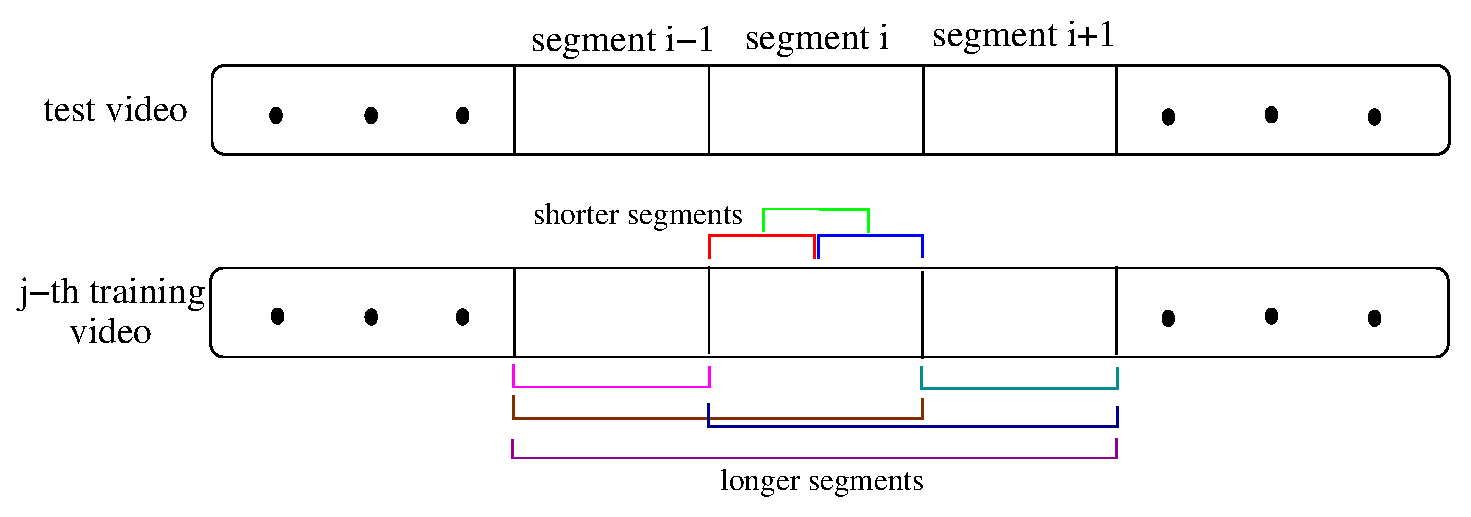
\epsfig{file=figures/mixture_of_segments.eps,width=1.0\linewidth}
  \end{center}
  \vspace{-4mm}
  \caption{An illustration of a mixture of segments with different temporal lengths
    and shifted temporal locations.}
  \vspace{-4mm}
  \label{fig:MSSC_illustration}
\end{figure}

More specifically, when calculating the likelihood of segment $i$ of the test
video, we not only take segment $(t_{i-1}, t_i]$ in the training video to
construct a basis, but also take $8$ segments in each training video to
construct $8$ more bases.  As illustrated in Fig.~\ref{fig:MSSC_illustration},
we take the $j$-th training video as an example.  These $8$ more segments are
$(t_{i-2}, t_{i-1}]$, $(t_i, t_{i+1}]$, $(t_{i-2}, t_i]$, $(t_{i-1}, t_{i+1}]$,
$(t_{i-2}, t_{i}]$, $(t_{i-1}, t_{i-1}+(t_i-t_{i-1})/2]$,
$(t_{i-1}+(t_i-t_{i-1})/2, t_i]$, and $(t_{i-1}+(t_i-t_{i-1})/4,
t_{i}-(t_i-t_{i-1})/4]$, which are all around segment $(t_{i-1}, t_i]$, but
with varied segment lengths and small temporal location shifts. We expect that
these additional bases can better handle the intra-class activity variation by
approximating the test video segments more accurately.

% =======================================================================================
\section{Experiments}\label{sec:experiments}

We test the proposed SC and MSSC methods on three human activity recognition
tasks: 1) the special case {\color{black}--} activity \textit{prediction},
where {\color{black}the} video gap is at the end of the video; 2) the general
case {\color{black}--} \textit{gapfilling}, where {\color{black}the} gap
separates two observed subsequences; and 3) the degenerate case
{\color{black}--} full video \textit{recognition}, where there is no gap along
the video. Each task is evaluated on real datasets with different challenge
levels. We implement the proposed methods in MATLAB, and use the Cuboids
descriptors~\cite{DollarVSPETS05cuboids} as spatiotemporal features. We use the
bag-of-visual-words technique to organize spatiotemporal features, in which a
codebook with $800$ words is generated by $K$-means clustering.  In
experiments, we consistently set $M=20$, i.e., each activity (and each video)
is uniformly divided into $20$ temporal segments.  We set $\sigma=6$ (in
Eqn.~(\ref{eq:likelihood_rewritten})) and $\lambda=10^{-2}$ (in
Eqn.~(\ref{eq:sparse_coding})) for the proposed methods throughout the three
recognition tasks.

We choose several state-of-the-art comparison methods, including Ryoo's human
activity prediction methods (both non-dynamic and dynamic
versions)~\cite{Ryoo2011}, early event detector -- MMED~\cite{MMED2012},
C2~\cite{Jhuang07abiologically}, and Action Bank~\cite{SaCoCVPR2012}.  Based on
their applicability, we apply these methods (adapted if necessary) on all or a
part of the three recognition tasks, which will be further explained in
following sections.  We also implement a baseline sparse coding (named after
`\textit{baseline}') method which concatenates features from different segments
of a training video into a single feature vector as one row of the basis matrix
and then directly applies sparse coding for recognition. More specifically, a
(partially observed) test video is classified into an activity class that leads
to the smallest reconstruction error.  Furthermore, in order to clarify that
the proposed SC and MSSC methods can perform better than voting methods which
share a similar idea of using a subset of training samples for classification,
we implement a KNN ($K$ Nearest Neighbor) algorithm as another comparison
method. Specifically, against each training video, we apply Ryoo's methods
(non-dynamic and dynamic versions) to calculate the posterior of the test
(partially observed) video and then identify the $K$ ($K$ is the number of
training videos in the same activity class) training videos against which the
test video has largest posteriors. This way, we can apply a simple majority
voting to the activity classes of $K$ nearest training videos to classify the
test video.

\subsection{Evaluation on the special case: prediction}

In the prediction task, we simulate incremental arrival of video frames
(represented by observation ratio $[0.1, 0.2, \dots, 1.0]$) as
in~\cite{Ryoo2011}, and evaluate the performance for each observation
ratio. Ryoo's methods, the KNN methods, MMED and the baseline sparse coding
method are selected for comparison since they can handle prediction.

For Ryoo's methods, since the original codes are not available publicly, we
implement them by following~\cite{Ryoo2011}. And by tuning parameters in our
implementation, we actually achieve comparable or even better performance than
those reported in~\cite{Ryoo2011}.  For MMED method, we use its published code
and follow the settings in~\cite{MMED2012}.  When recognizing a test video
$\mathcal{O}$, it is concatenated with other test videos from other activity
classes into a long video, with $\mathcal{O}$ at the end. MMED returns a
subsequence in this long video.  To adapt MMED from early event detection to
human activity prediction, we set its minimum searching length to be the
temporal length of $\mathcal{O}$, and the step length of the searching to be
identical to the segment length in the proposed SC method.  If the subsequence
returned by MMED contains no less than $50\%$ of the frames in the observed
subsequence in $\mathcal{O}$, it is counted as a correct prediction.

We have three datasets for evaluating prediction: \textit{UT-interaction \#1},
\textit{UT-interaction \#2}~\cite{UT-Interaction-Data} and \textit{DARPA Y1}, a
subset of videos from the Year-1 corpus of the DARPA Mind's Eye
program~\cite{Darpa-dataset}.  In DARPA Y1, each video shows one of the $7$
human activities: `fall', `haul', `hit', `jump', `kick', `push' and `turn'.
For each activity class, we collect $20$ videos.
% As partly illustrated in Fig.~\ref{fig:Darpa_dataset_challenges},
DARPA Y1 is much more complex than the UT-interaction datasets in that 1)
{\color{black}actor size} in the same activity class varies significantly in
different videos; 2) the overhead time for an activity varies from one video to
another; 3) activities are recorded from different camera perspectives; 4)
activity pace varies in different videos; and 5) backgrounds are more complex
due to shadows and non-uniform illuminations.

As in~\cite{Ryoo2011}, we use the leave-one-out cross validation for
performance evaluation.  There are $10$ folds of cross validations on
UT-interaction \#1, \#2; $20$ folds of cross validations on DARPA Y1.  For each
test video, the result is a single human activity class out of all possible
activities classes and we use the average accuracy over all cross validation
tests and all activity classes as a quantitative metric of the performance.
\begin{figure*}[htbp]
  \centering
  \subfigure[]{
    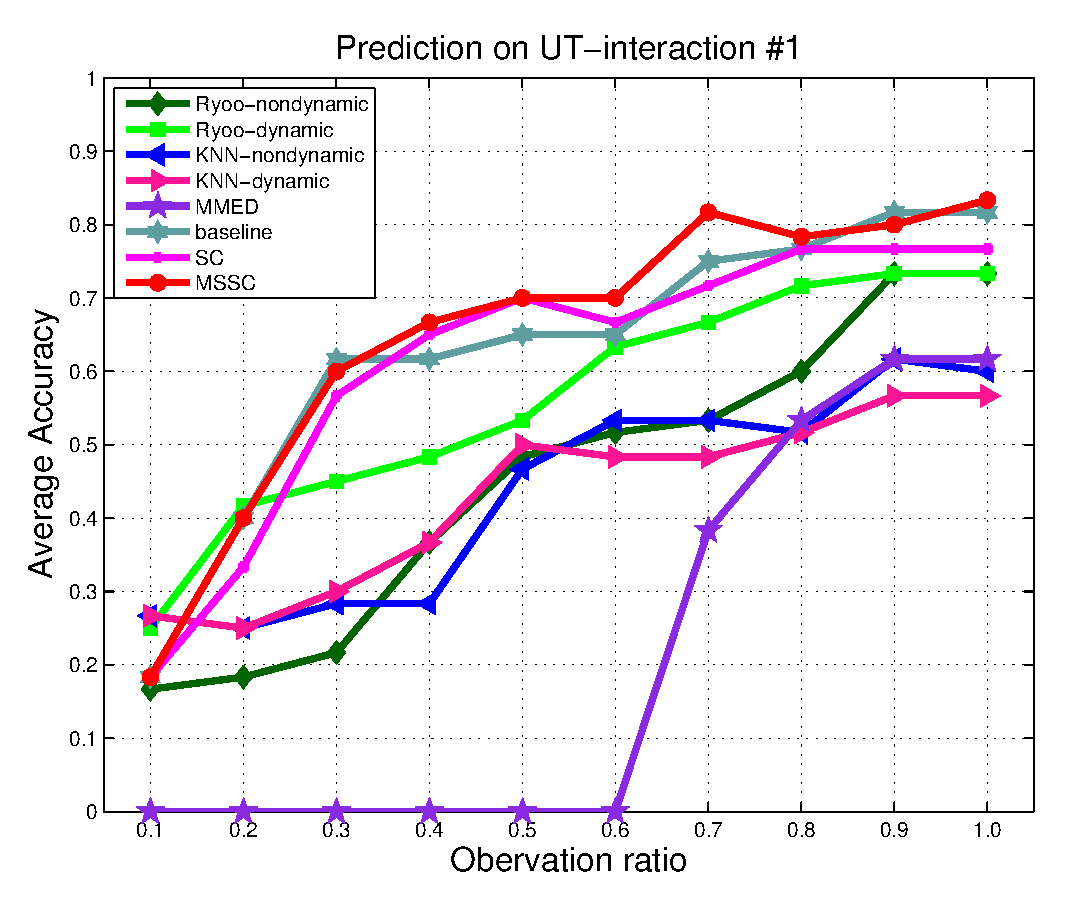
\includegraphics[width=0.31\textwidth]{figures/prediction/UT-interaction_1.eps}
  }
  \subfigure[]{
    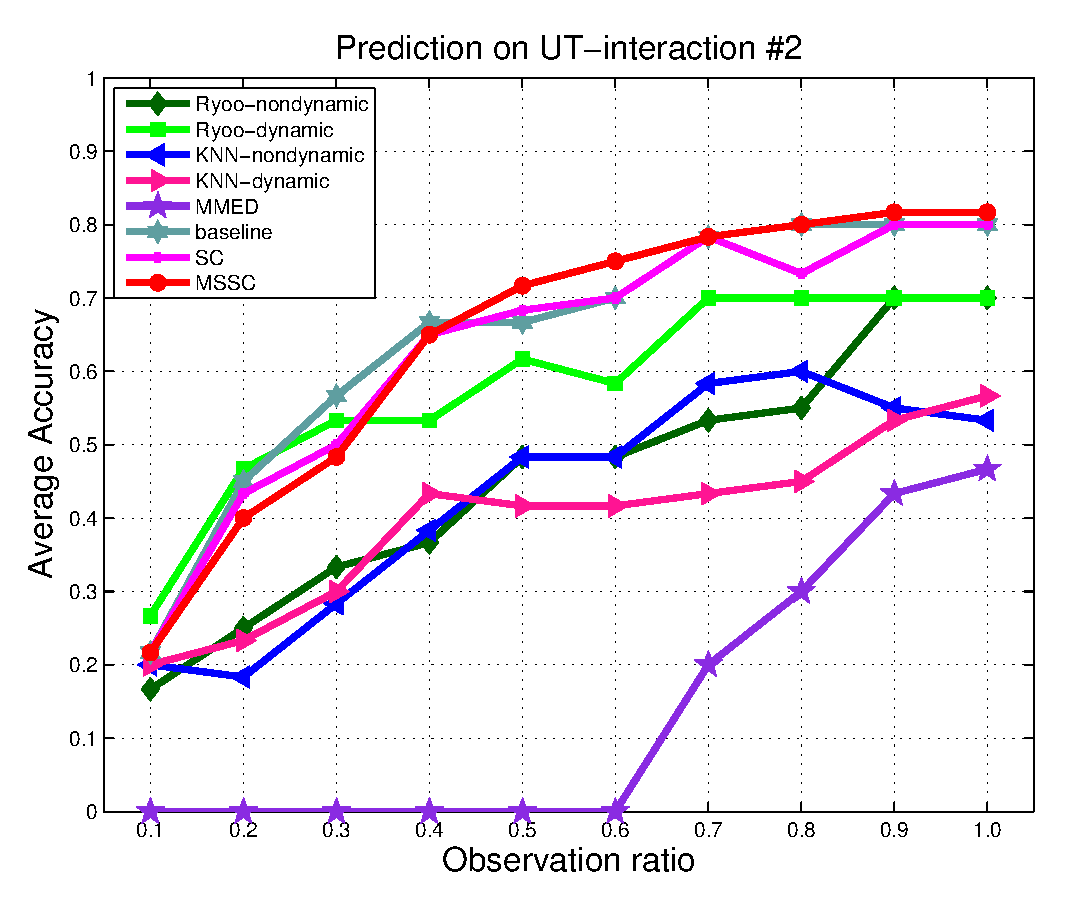
\includegraphics[width=0.31\textwidth]{figures/prediction/UT-interaction_2.eps}
  }
  \subfigure[]{
    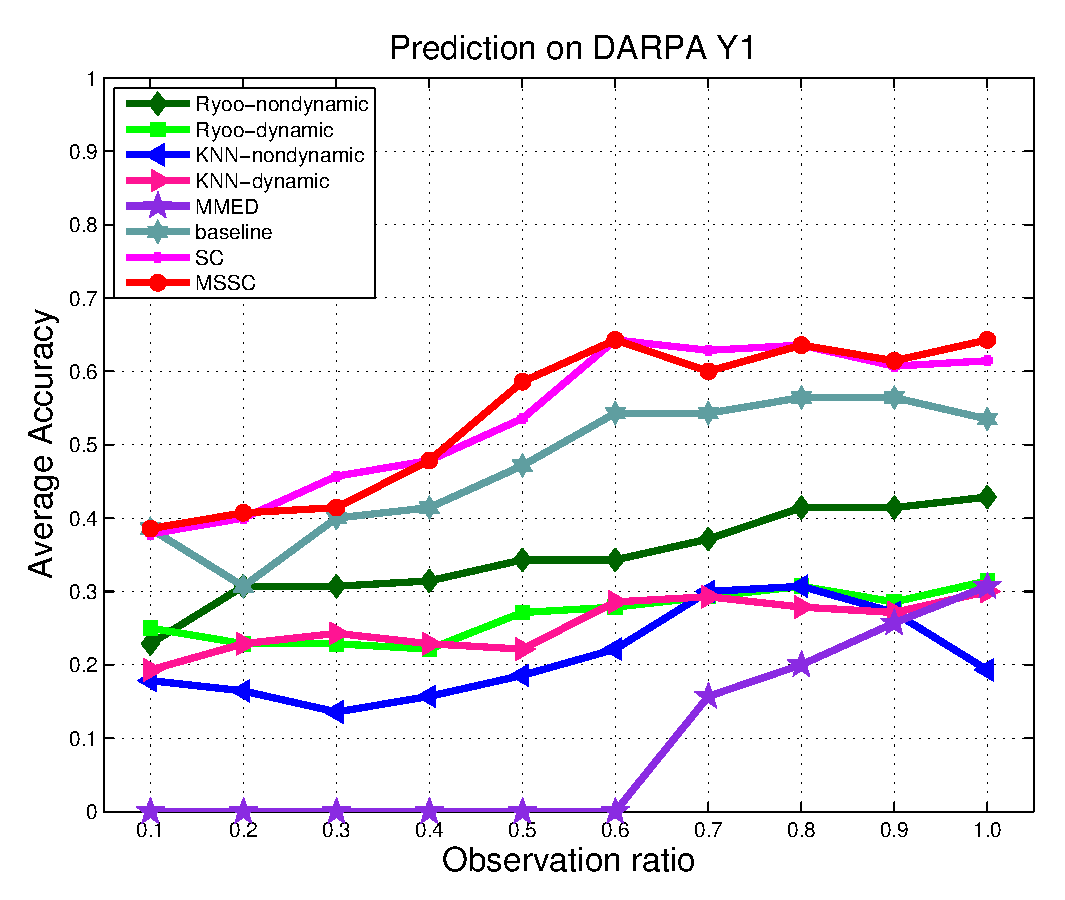
\includegraphics[width=0.31\textwidth]{figures/prediction/darpaY1.eps}
  }
  \caption{Prediction results on three datasets: (a) UT-interaction \#1; (b) UT-interaction \#2; and (c) DARPA Y1.}
  \vspace{-4mm}
  \label{fig:prediction_results}
\end{figure*}

Figure~\ref{fig:prediction_results} shows {\color{black}the prediction results}
on these three test datasets.  We can see that, the proposed SC and MSSC
methods show comparable or better performance on these three datasets,
especially on DARPA Y1 and when the observation ratio is not overly small.  The
baseline sparse coding method achieves good performance (close to SC and MSSC)
on UT-interaction \#1, \#2 but not in DARPA Y1 because the activities in
UT-interaction datasets show very small intra-class variations, while the
proposed methods can better handle the large intra-class variations. MMED
performs not as good as other methods because MMED is originally designed for
early event detection, with a goal of localizing the starting and ending frames
of an activity and this is different from the prediction task in this
experiment, where our goal is to recognize the activity from a given observed
subsequence.

\subsection{Evaluation on the general case: gapfilling}
In the gapfilling task, we compare the proposed SC and MSSC methods with
adapted Ryoo's methods (non-dynamic and dynamic versions), KNN (non-dynamic and
dynamic versions) and the baseline sparse coding method. Specifically, we adapt
Ryoo's methods to perform activity prediction on these two subsequences, and
the gapfilling posterior score is the summation of prediction posterior scores
on each observed subsequence. We use the same parameter setting for adapted
Ryoo's methods as used in the prediction task.

We first perform gapfilling evaluation on UT-interaction \#1,\#2 and DARPA Y1
datasets.  We intentionally replace a subsequence of frames from a test video
by empty frames to create a partially observed video. To have a more reliable
performance evaluation, we try different lengths and different temporal
locations of empty subsequences for each test video. Specifically, for each
test video $\mathcal{O}[1:T]$, we construct a non-observation interval
$(\beta_1T:\beta_2T]$, where
\begin{equation}
  \label{eq:gap_setting}
  (\beta_1, \beta_2) = \{[0.1, 0.2, \cdots, 0.9] \times [0.2, 0.3, \cdots, 0.9]\},
\end{equation}
and $\beta_1 < \beta_2$. We further define non-observation ratio as
$\hat{\beta} = \beta_2-\beta_1$ which varies from $0.1$ to $0.8$ with the step
of $0.1$ according to Eqn.~(\ref{eq:gap_setting}). We finally evaluate the
accuracy rate in {\color{black}term} of each possible non-observation ratio
$\hat{\beta}$ by counting the percentage of the correctly recognized test
videos with the non-observation ratio $\hat{\beta}$ over all folds ($10$ folds
for UT-interaction \#1, \#2; $20$ folds for DARPA Y1) of cross validations.

As shown in Fig.~\ref{fig:gapfilling_comparison_single_verb}, we achieve a
similar performance ranking as in the prediction evaluations. The proposed SC
and MSSC methods achieve comparable or better performance when
{\color{black}the} gap ratio is not overly large. On the more complex DARPA Y1
dataset, the proposed methods clearly achieve better performance.

\begin{figure*}[htbp]
  \centering
  \subfigure[]{
    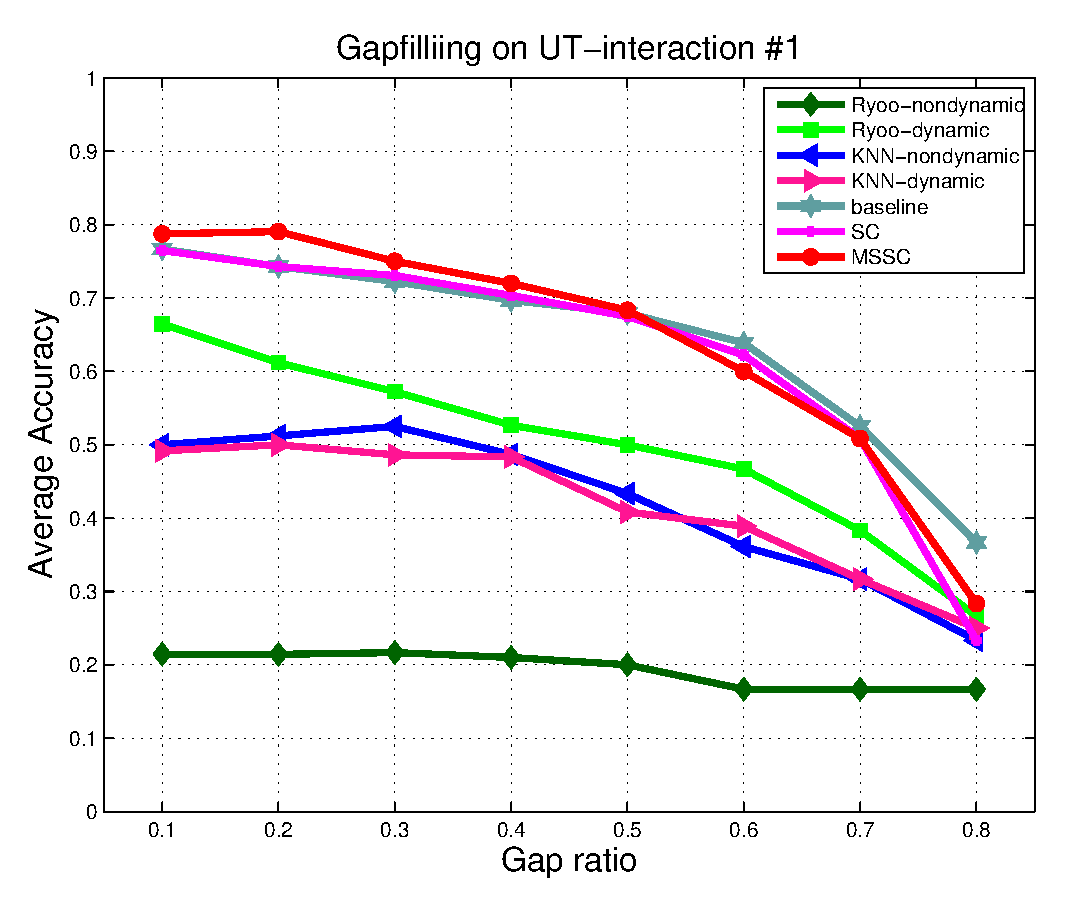
\includegraphics[width=0.31\textwidth]{figures/gapfilling/UT-interaction_1.eps}
  }
  \subfigure[]{
    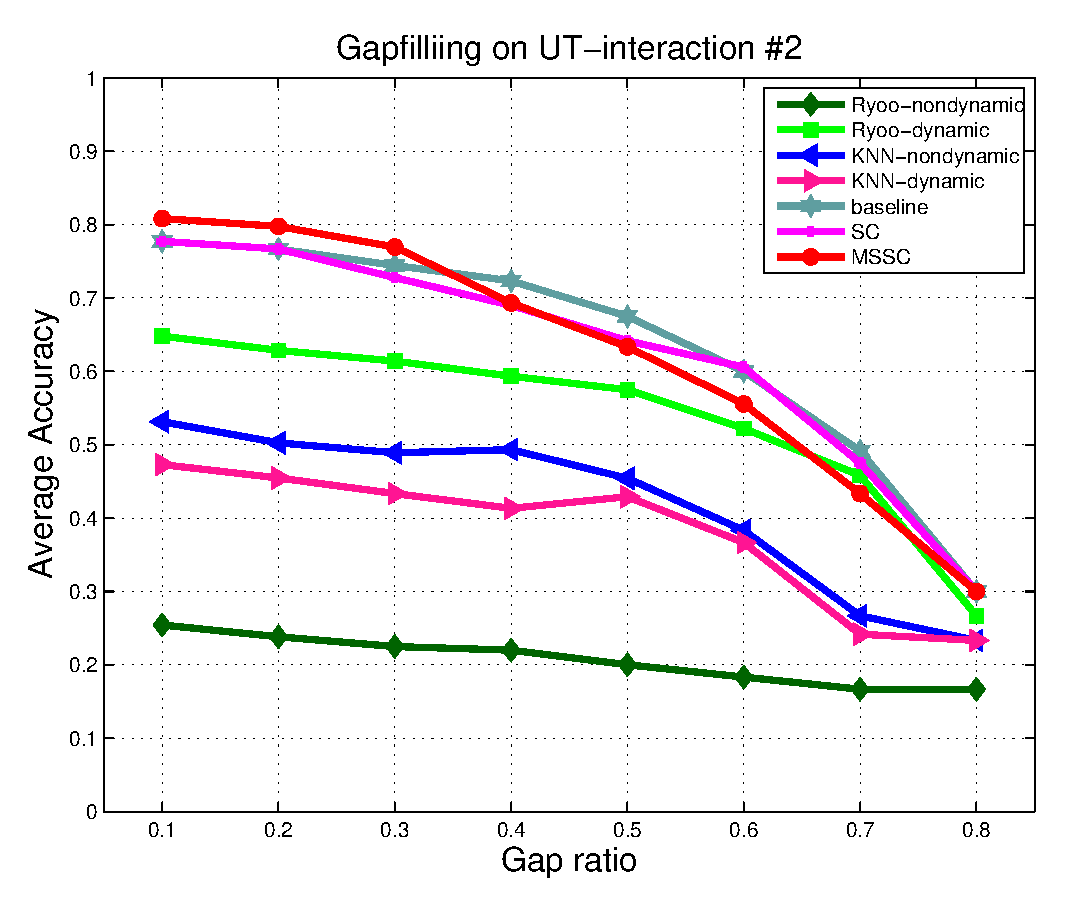
\includegraphics[width=0.31\textwidth]{figures/gapfilling/UT-interaction_2.eps}
  }
  \subfigure[]{
    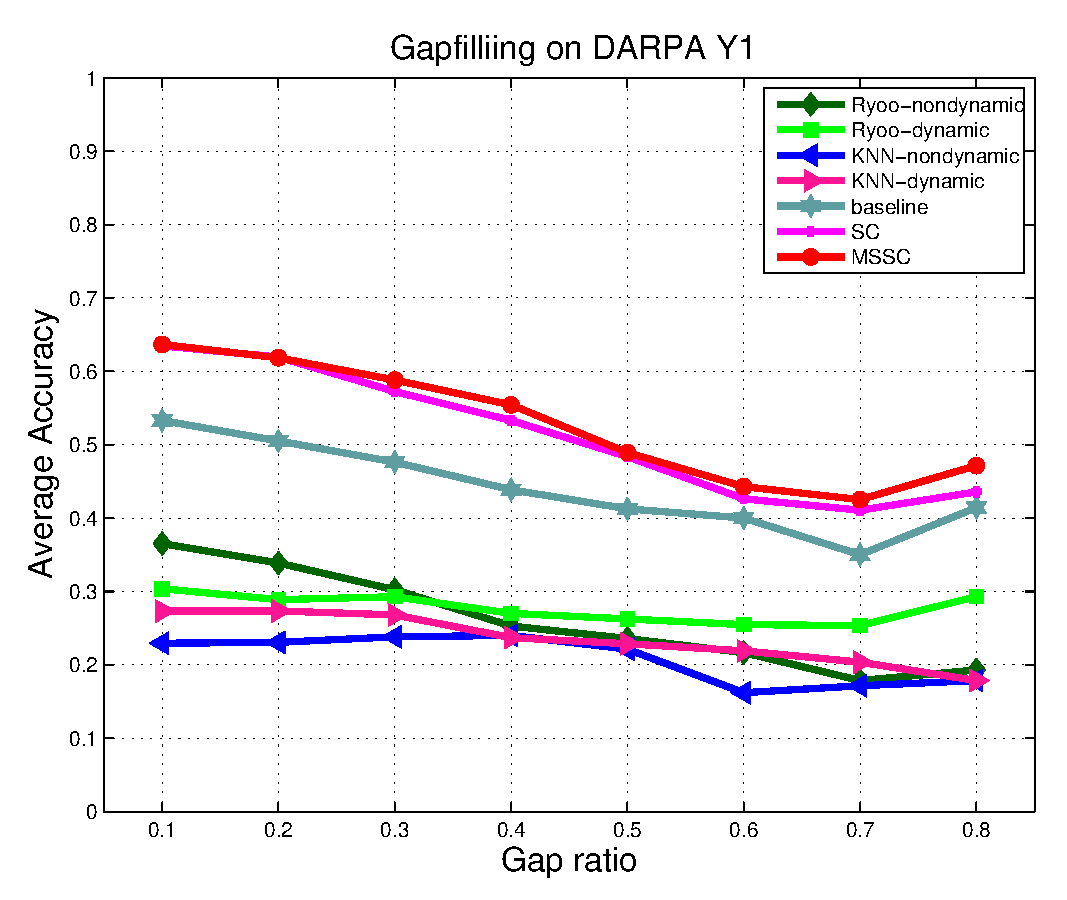
\includegraphics[width=0.31\textwidth]{figures/gapfilling/darpaY1.eps}
  }
  \caption{Gapfilling results on three datasets: (a) UT-Interaction \#1; (b)
    UT-interaction \#2; and (c) DARPA Y1.}
  \vspace{-2mm}
  \label{fig:gapfilling_comparison_single_verb}
\end{figure*}

We further evaluate the proposed methods and comparison methods on more complex
datasets: The DARPA Mind's Eye program provides a Year-2 evaluation corpus,
which contains $4$ sub-datasets of long test videos (each video has a length
more than ten minutes) with multiple gaps. For brevity, we name this dataset as
\textit{DARPA Y2-Gapfilling} and the four sub-datasets are `gapfilling short
duration', `gapfilling long duration',`gapfilling natural description', and
`gapfilling natural recognition', respectively. This dataset is much more
challenging than DARPA Y1 dataset due to: 1) the important action units are
missing for the underlying activities in many cases; and 2) many activities are
performed simultaneously by multiple actors. In DARPA Y2-Gapfilling, there are
in total $267$ gaps, with length from $122$ to $2,239$ frames.

DARPA Mind's Eye program also provides three training sets (different from
DARPA Y2-Gapfilling) to learn the model for each activity.  These three
training sets are `C-D2b' ($22$ activity classes, totally $3,819$ training
videos), `C-D2c' ($16$ activity classes, totally $2,80$ training videos) and
`C-D2bc' ($23$ activity classes, totally $4,409$ training videos).  We perform
the proposed and comparison methods on all videos in DARPA Y2-Gapfilling with
respect to these three training datasets, respectively. In our experiment, for
each gap in DARPA Y2-Gapfilling, we construct test video clips by including a
certain number of observed frames before and/or after this gap. For each gap,
nine video clips are constructed with the gap appearing `at the beginning', `in
the center' or `at the end' of the video clip and counting for $20\%$, $40\%$
or $60\%$ of the clip length. This way, we construct a total of $2,403$ video
clips with a gap and evaluate the recognition results against the human
annotated ground-truth (may give multiple activities labels for a test gapped
video clip). Precision-recall results (obtained by thresholding the posteriors)
are shown in Fig.~\ref{fig:gapfilling_comparison_multiple_verb}. We can see
that the proposed SC and MSSC methods outperform the comparison methods in most
of the test clips. However, the general performance is low, which indicates
that the gapfilling on practical scenarios is far from a solved problem.

\begin{figure*}[htbp]
  \begin{center}
    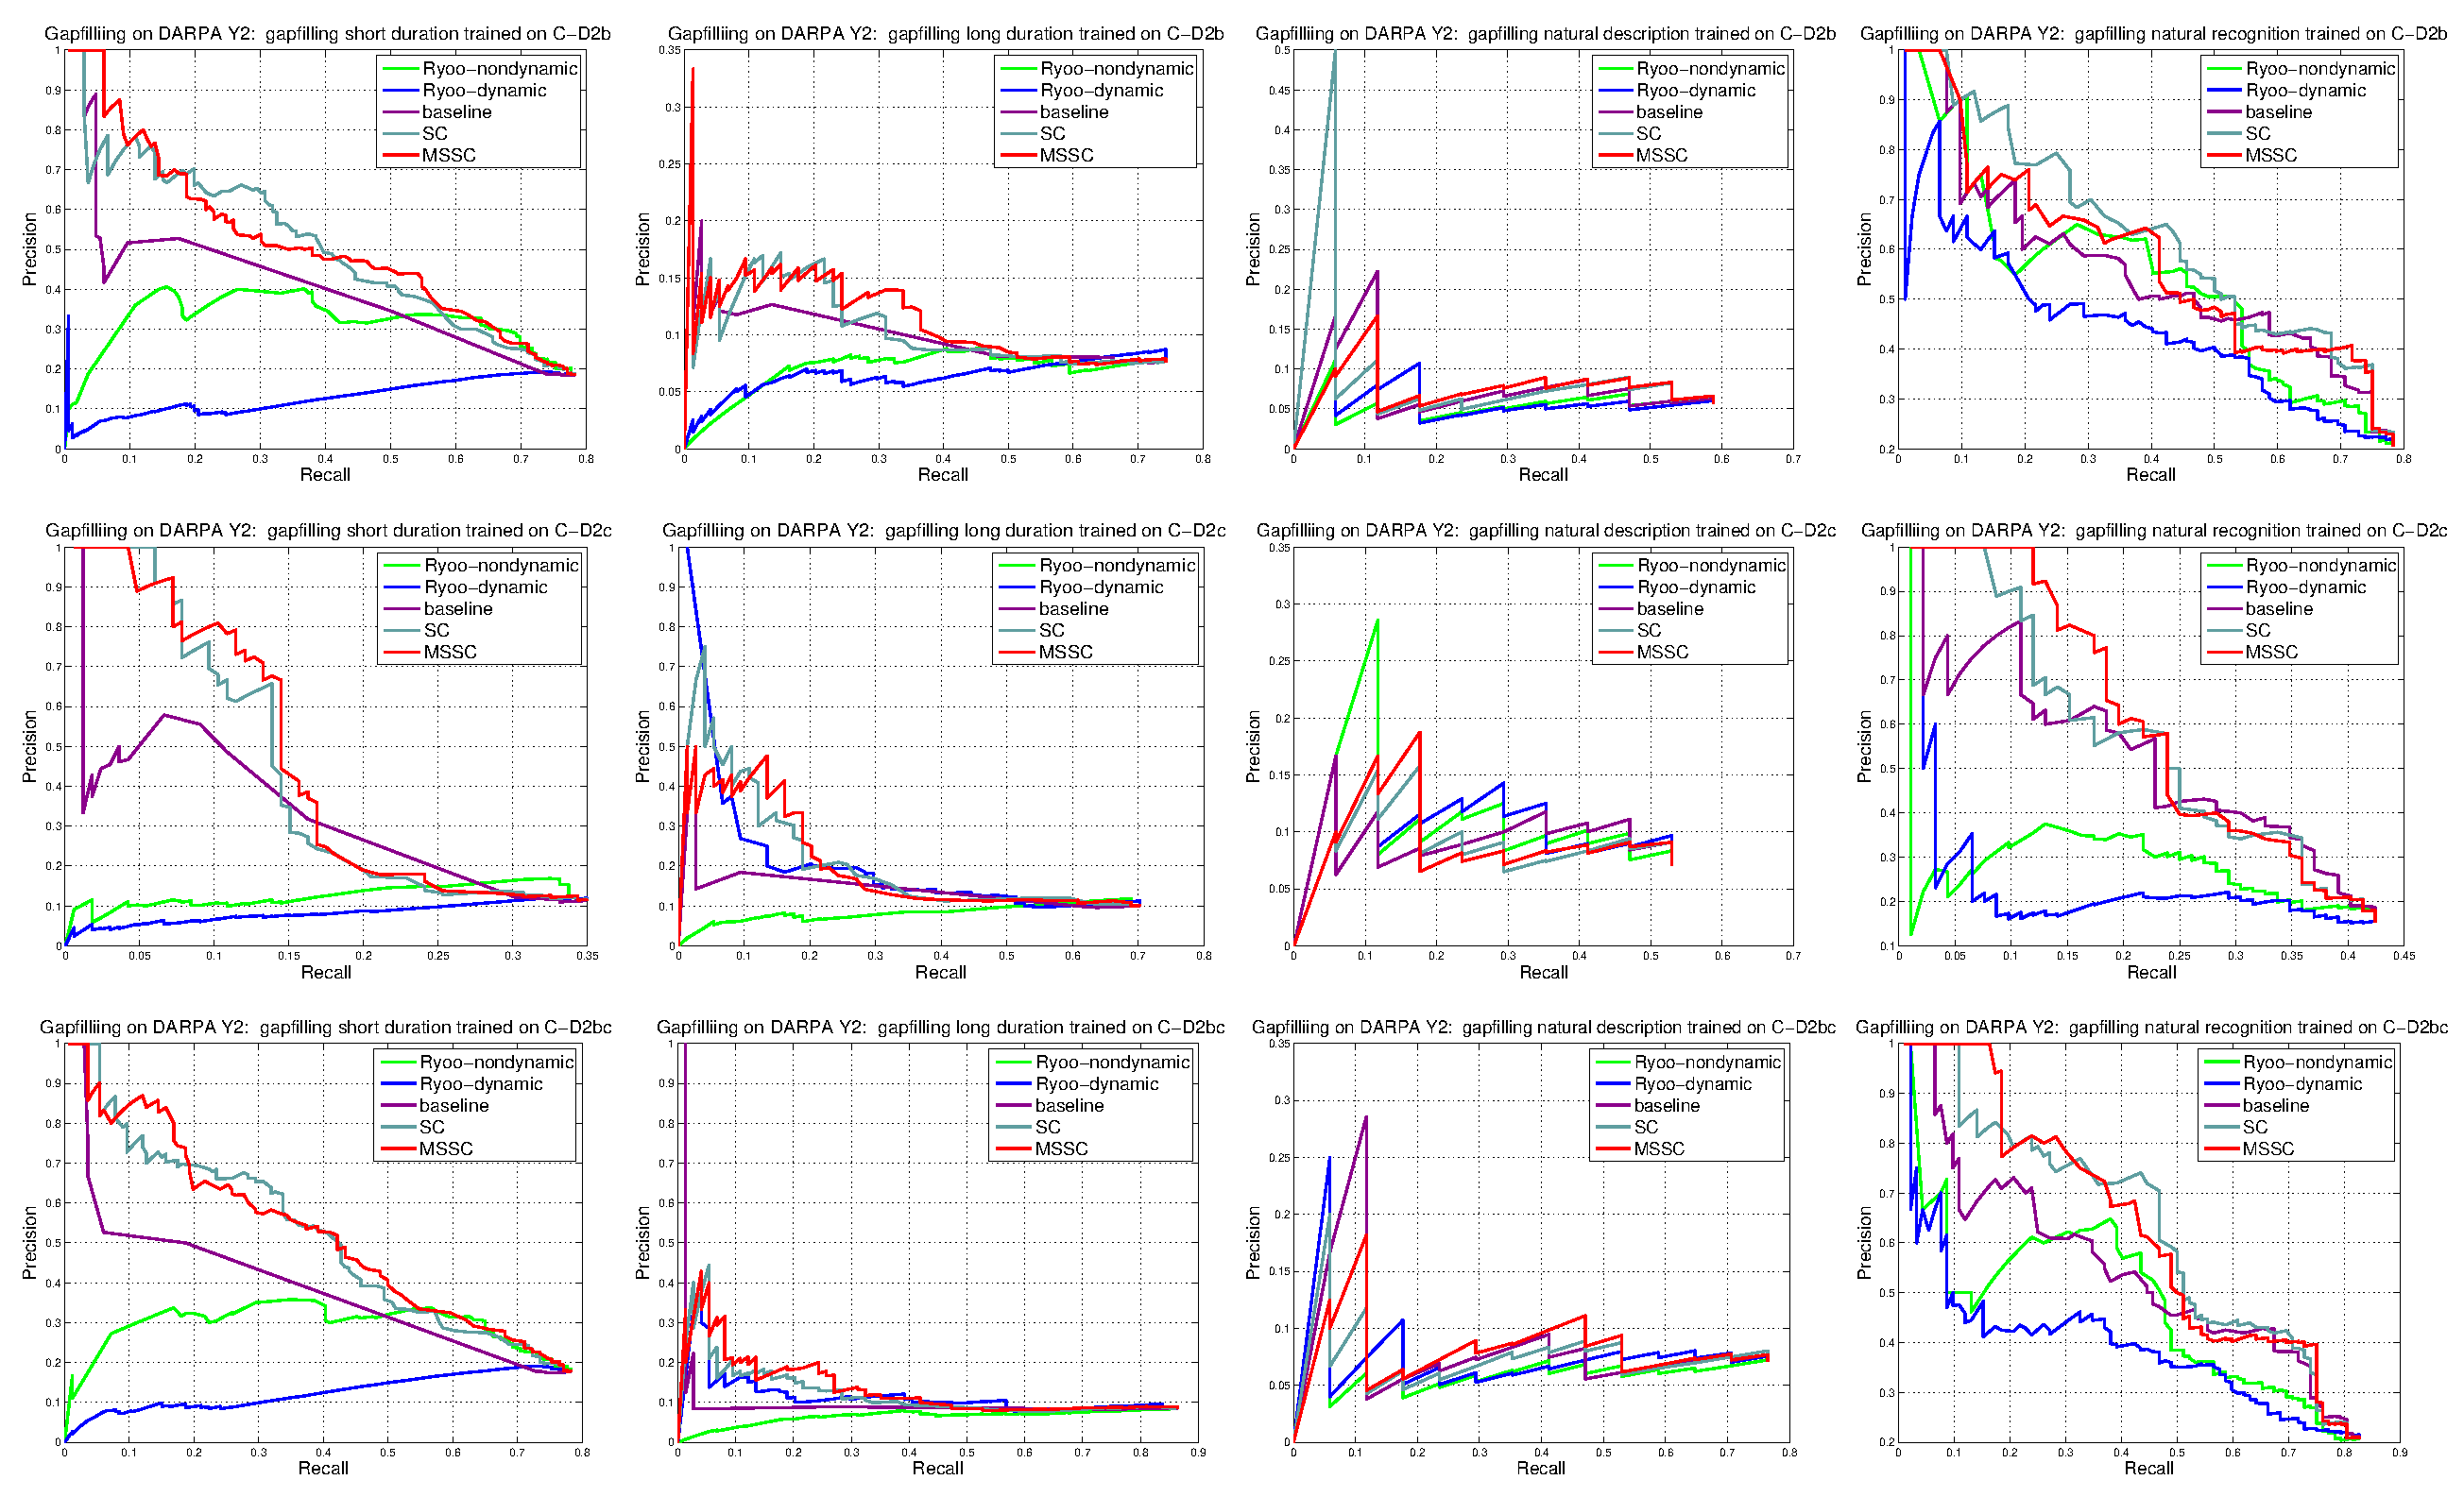
\epsfig{file=figures/gapfilling_comparison_multiple_verb.eps, width=1.0\linewidth}
  \end{center}
  \vspace{-4mm}
  \caption{Gapfilling results on DARPA Y2-Gapfilling dataset. Row 1, 2 and 3 show the results by training on `C-D2b',
    `C-D2c' and `C-D2bc', respectively. Column 1, 2, 3 and 4 show the results on `gapfilling short duration', `gapfilling long duration',
    `gapfilling natural description', and `gapfilling natural recognition', respectively.}
  \vspace{-4mm}
  \label{fig:gapfilling_comparison_multiple_verb}
\end{figure*}

\subsection{Evaluation on degenerate case: full-video recognition}

For full-video recognition, we compare the proposed SC and MSSC methods with
the baseline sparse coding, Ryoo's methods (non-dynamic and dynamic versions),
C2 and Action Bank.  Previous published recognition methods are mostly
evaluated on short video clips where each of them contains a single activity,
which cannot reflect {\color{black}real performance} in the practical
scenarios.  Thus, besides the full video recognition results on UT-interaction
\#1,\#2 and DARPA Y1 provided in prediction task (see
Fig.~\ref{fig:prediction_results} at observation ratio $1.0$), we further test
these methods on \textit{DARPA Year-2 Recognition}, a dataset provided by the
DARPA Minds' Eye program for large-scale activity recognition evaluation. DARPA
Year-2 Recognition contains $3$ sub-datasets: `description free form',
`description scripted', and `recognition'. DARPA Y2-Recognition is very
challenging because 1) the length of each video is around (mostly larger than)
ten minutes (more than one and half hours in total); and 2) a large number of
subsequences contain unrelated moving objects in the background.

We break the long video into partially overlapping short clips using sliding
windows for activity recognition. For the proposed SC and MSSC methods, Ryoo's
methods (non-dynamic and dynamic versions), and the baseline sparse coding
method, we calculate the posteriors {\color{black}of each activity presented in
  each short clip}. We normalize the posterior scores that an activity is
present in each short clip and label the video clip with the activities that
have posterior scores larger than a pre-set threshold $\tau$. In the
experiments, we choose $\tau= 0.05$ and C-D2b as the training set.  For C2 and
Action Bank methods, we use their default parameters to detect activities in
each constructed video clip. We check the overlap between the sliding window
with the recognized activities and the ground-truth labeling of the activities
(starting and ending frames) using the intersection/union ratio. Given the
identical activity label, we threshold this overlap ratio to get
precision/recall values and then combine them into a $F_1$-measure, which is
shown in Table~\ref{tab:recognition_comparison}. As shown in the table, the
proposed SC, MSSC and baseline sparse coding methods achieve relatively better
performance on two different ground-truth labelings. However, the general
performance is very low and this indicates that there is still a long way to go
to achieve good activity recognition in practical scenarios.
\begin{table*}[htbp]
  \begin{center}
    \resizebox{0.95\linewidth}{!}{
      \begin{tabular}{c||c|c|c|c|c|c|c|c|c|c|c|c}
        \hline\hline
        \multicolumn{13}{c}{$F_1$-measures evaluated against ground-truth I} \\
        \hline
        Test datasets & \multicolumn{4}{c|}{`description free form'} &\multicolumn{4}{c|}{`description scripted'} & \multicolumn{4}{c}{`recognition'} \\
        \hline
        Overlap thresholds & 0.4 & 0.5 & 0.6 & 0.7 & 0.4 & 0.5 & 0.6 & 0.7 & 0.4 & 0.5 & 0.6 & 0.7\\
        \hline
        Ryoo's dynamic 		& $0.81\%$ 	& $0.68\%$ 	& $0.54\%$ 	& $0.33\%$ 	& $8.6\%$ 	& $8.6\%$ 	& $8.6\%$ 	& $8.6\%$ 	& $0.9\%$ 	& $0.67\%$ 	& $0.49\%$ 	& $0.28\%$\\
        Ryoo's non-dynamic 	& $0\%$ 	& $0\%$ 	& $0\%$ 	& $0\%$ 	& $0\%$ 	& $0\%$ 	& $0\%$ 	& $0\%$ 	& $0\%$ 	& $0\%$ 	& $0\%$ 	& $0\%$\\
        baseline & $\textbf{1.24\%}$ & $\textbf{1.11\%}$ & $\textbf{0.83\%}$ 	& $\textbf{0.53\%}$ 	& $15.45\%$ & $15\%$ 	& $14.09\%$ & $13.64\%$ & $\textbf{1.09\%}$ 	& $0.89\%$ 	& $0.72\%$ 	& $0.48\%$\\
        MSSC 				& $1.04\%$ 	& $0.92\%$ 	& $0.71\%$ 	& $0.46\%$ 	& $10.97\%$ & $10.97\%$ & $10.47\%$ & $9.98\%$ 	& $1\%$ 	& $0.84\%$ 	& $0.68\%$ 	& $0.45\%$\\
        SC  & $1.23\%$ 	& $1.10\%$ 	& $0.82\%$ 	& $\textbf{0.53\%}$ & $\textbf{16.39\%}$ & $\textbf{15.85\%}$ & $\textbf{14.75\%}$ & $\textbf{14.21\%}$ & $\textbf{1.09\%}$ & $\textbf{0.90\%}$ & $\textbf{0.75\%}$ & $\textbf{0.5\%}$\\
        C2 			& $0.52\%$ 	& $0.26\%$ 	& $0.26\%$ 	& $0.26\%$ 	& $0\%$ 	& $0\%$ 	& $0\%$ 	& $0\%$ 	& $0\%$ 	& $0\%$ 	& $0\%$ 	& $0\%$\\
        Action Bank 		& $0.38\%$ 	& $0\%$ 	& $0\%$ 	& $0\%$ 	& $0.53\%$ 	& $0.18\%$ 	& $0.18\%$ 	& $0.18\%$ 	& $0.25\%$ 	& $0.25\%$ 	& $0.25\%$ 	& $0.25\%$\\
        \hline\hline
        \multicolumn{13}{c}{$F_1$-measures evaluated against ground-truth II} \\
        \hline
        Test datasets & \multicolumn{4}{c|}{`description free form'} &\multicolumn{4}{c|}{`description scripted'} & \multicolumn{4}{c}{`recognition'} \\
        \hline
        Overlap thresholds & 0.4 & 0.5 & 0.6 & 0.7 & 0.4 & 0.5 & 0.6 & 0.7 & 0.4 & 0.5 & 0.6 & 0.7\\
        \hline
        Ryoo's dynamic & $0.77\%$ & $0.66\%$ & $0.49\%$ & $0.26\%$ & $6.52\%$ & $4.35\%$ & $4.35\%$ & $4.35\%$ & $0.98\%$ & $0.74\%$ & $0.52\%$ & $0.29\%$\\
        Ryoo's non-dynamic & $0\%$ & $0\%$ & $0\%$ & $0\%$ & $0\%$ & $0\%$ & $0\%$ & $0\%$ & $0\%$ & $0\%$ & $0\%$ & $0\%$\\
        baseline & $0.93\%$ & $\textbf{0.8\%}$ & $\textbf{0.65}\%$ & $0.41\%$ & $6.83\%$ & $6.38\%$ & $5.92\%$ & $5.47\%$ & $\textbf{1.14\%}$ & $\textbf{0.99\%}$ & $\textbf{0.8\%}$ & $\textbf{0.51\%}$\\
        MSSC & $0.85\%$ & $0.72\%$ & $0.56\%$ & $0.37\%$ & $6\%$ & $5.5\%$ & $5.5\%$ & $5\%$ & $1.06\%$ & $0.93\%$ & $0.74\%$ & $0.46\%$\\
        SC & $0.91\%$ & $\textbf{0.8}\%$ & $\textbf{0.65\%}$ & $\textbf{0.42\%}$ & $\textbf{7.12\%}$ & $\textbf{6.58}\%$ & $\textbf{6.03}\%$ & $\textbf{5.48}\%$ & $1.13\%$ & $\textbf{0.99\%}$ & $\textbf{0.8\%}$ & $0.5\%$\\
        C2 & $\textbf{0.97\%}$ & $0.32\%$ & $0\%$ & $0\%$ & $5.26\%$ & $5.26\%$ & $3.51\%$ & $1.75\%$ & $0\%$ & $0\%$ & $0\%$ & $0\%$\\
        Action Bank & $0.67\%$ & $0.67\%$ & $0.22\%$ & $0\%$ & $0.78\%$ & $0.59\%$ & $0.39\%$ & $0.2\%$ & $0.72\%$ & $0.48\%$ & $0.48\%$ & $0.24\%$\\
        \hline\hline
      \end{tabular}}
  \end{center}
  \caption{Recognition results on DARPA Y2-Recognition dataset. The best $F_1$-measures on each test dataset at each
    overlap threshold are highlighted. The top and bottom tables show the results
    on two different sets of ground-truth labeling constructed manually.}
  \label{tab:recognition_comparison}
\end{table*}

% =======================================================================================
\vspace{-3mm}
\section{Conclusion}\label{sec:conclusion}
In this paper, we proposed novel methods for recognizing human activities from
partially observed videos. We formulated the problem as a
posterior-maximization problem whose likelihood is calculated on each activity
temporal {\color{black}stage} using a sparse coding (SC) technique. We further
include more sparse coding bases for a mixture of varied-length and/or
varied-location segments (MSSC) from the training videos. We evaluated the
proposed SC and MSSC methods on three tasks: activity prediction, gapfilling
and full-video recognition.  The experimental results demonstrate that the
proposed methods produce better {\color{black}performance} than many
state-of-the-art methods when the test datasets are complex. In contrast to
many previous approaches, we conducted experiments on complex datasets that
reflect practical scenarios. The results show that there is still a long way to
go to achieve satisfactory recognition on such data.
